\defaultfont
\chapter{接收机系统设计}

\section{MSP432扩频接收机软件设计}
\subsection{MSP432驱动程序设计}
	MSP432驱动程序包括ADC数据采集驱动和UART数据传输驱动两部分。
在设计驱动程序时参考了中断-回调函数模型,即中断服务函数处理中断请求然后请求调用
回调函数。回调函数不是由中断服务函数直接调用,而是由中断服务函数连接到回调函数链表中由
主函数根据优先级决定执行哪个回调函数。

	下面结合这一模型及具体驱动程序做详细说明。

\subsubsection{ADC数据采集驱动}
	系统采用带通采样以降低数据处理负荷,采样率$4KHz$。MSP432的Timer\_A0为ADC14提供采样率
的采样保持时钟。为保证系统实时性,采集数据设计为PING-PONG存储。MSP432的$\mu$DMA模块提供这一功能。
PING-PONG大小为$2\times1024$存储单元。每采集完成一次PING-PONG即触发一次中断,在中断服务函数中判断
是PING还是PONG,然后请求调用回调函数。

	回调函数的形式为:void msp432\_adc14\_callback(uint16\_t *data, uint32\_t len)。
参数data为当前完成采集的存储区的首地址,参数len为存储区大小。图\ref{Figure:Software:ADCModule}为ADC数据采集驱动的流程图。
	% 流程图定义基本形状
	\tikzstyle{startstop} = [rectangle, rounded corners, minimum width=3cm, minimum height=1cm,text centered, draw=black]
	\tikzstyle{io} = [trapezium, trapezium left angle=70, trapezium right angle=110, minimum width=3cm, minimum height=1cm, text centered, draw=black]
	\tikzstyle{process} = [rectangle, minimum width=3cm, minimum height=1cm, text centered, draw=black]
	\tikzstyle{decision} = [diamond, minimum width=3cm, minimum height=1cm, text centered, draw=black]
	\tikzstyle{arrow} = [thick,->,>=stealth]
	\begin{figure}[htbp]
		\centering
		\begin{tikzpicture}[node distance=2.0cm]
		%定义流程图具体形状
		\node (start) [startstop] {中断触发};
		\node (dec1) [decision, below of=start, yshift=-1.5cm] {PING中断?};
		\node (dec2) [decision, below of=dec1, yshift=-2.5cm] {PONG中断?};
		\node (pro1) [process, right of=dec2, xshift=2.5cm] {请求回调};
		\node (return) [startstop, below of=dec2,yshift=-1.5cm] {返回};
		\path node(fake) [right of=pro1]{};
		
		
		%连接具体形状
		\draw [arrow](start) -- (dec1);
		\draw [arrow](dec1) -| node[anchor=south] {是} (pro1);
		\draw [arrow](dec1) -- node[anchor=east] {否} (dec2);
		
		\draw [arrow](dec2) -- node[anchor=north] {是} (pro1);
		\draw [arrow](dec2) -- node[anchor=east] {否} (return);
		
		\draw [arrow](pro1) |-  (return);
		\end{tikzpicture}
		\caption{ADC数据采集驱动流程图}
		\label{Figure:Software:ADCModule}
	\end{figure}

\subsubsection{UART数据传输驱动}
	UART驱动设计为1152008N1(波特率115200bps,8位数据位,无校验位,1位停止位)传输格式。UART的接受
采用中断-回调函数模型,回调函数形式为:void msp432\_uart\_callback(uint16\_t *data, uint32\_t len)。

	UART的发送利用$\mu$DMA以实现非阻塞调用。提供给的外部编程接口为函数int msp432\_uart\_send(uint8\_t *data, uint32\_t len)
,函数将数据存入缓存区域并启动uDMA通道。函数返回实际写入缓存区域的数据长度,如果写入失败则返回-1。 

\subsection{MSP432动态内存管理}
	单片机在做信号处理算法时常常遇到需要使用较大数组的问题。例如在做32bit浮点采样数据为900点,本地数据为108点的快速相关算法时
需要分配至少两个4k大小的存储区域。在编写函数时有三种处理方式:

\begin{publist}
	\item 使用全局变量静态分配内存,存储区位于静态数据区。这样做的好处是分配内存在程序便以阶段就已经做好,但是内存永久占用不能释放,而且对于内存较小的
	单片机来说,分配较多的大块内存将带来大量内存的消耗;
	\item 使用局部变量,存储区位于栈内。这样做可以函数调用完之后内存可以释放,可以缓解静态分配内存的问题。但是如果遇到函数多次嵌套调用可能会导致栈益处;
	\item 使用malloc动态分配内存,存储区位于堆内。这样做可以解决静态分配和局部变量动态分配的所有问题,但是c标准库中的malloc函数算法复杂,分配与释放
	很耗时,而且需要链接较大的标准库的代码使程序体积增大。
\end{publist}

	信号处理算法虽然需要较多的大块内存,但是所有的内存大小几乎都一致即对某个固定大小的内存需求较多。针对这一前提,并结合动态内存分配的内存池算法重新实现了
快速的动态内存管理。


\subsubsection{内存池介绍}
	内存池(Memory Pool),又被称为固定大小区块规则(fixed-size-block allocation),允许程序设计者以类似C语言的malloc或者C++的new运算符进行动态内存的申请。
对于其他动态内存分配算法来说,因为会动态记忆区块大小导致的碎片问题,致使在实时系统上表现不佳,甚至根本无法使用。
内存池技术提供了一种更有效率的解决方案:预先规划一定数量的内存区块,使程序可以在执行期分配(allocate)、使用(access)和释放(free)内存区块。
	
	图\ref{Figure:Software:memalloc}为以内存池实例,内存池包含4个1k大小、2个2k大小和1个4k大小的内存块。图\ref{Figure:Software:memalloc}还展示了多次分配内存的过程:
	
\begin{publist}
	\item 请求一个大小为4k的内存快,此时内存池匹配到第一个大小为2k的内存区域;
	\item 请求4个大小都为1k的内存快,此时内存池分别匹配到4个大小为1k的内存区域,至此大小为1k的内存块用尽;
	\item 再次请求一个大小为1k的内存块,此时内存池将在2k大小的池内匹配内存区域
	\item 如果再请求1k或者2看的内存块,内存池将在4k大小的池内匹配内存区域。
\end{publist}
	\begin{figure}[htbp]
		\centering
		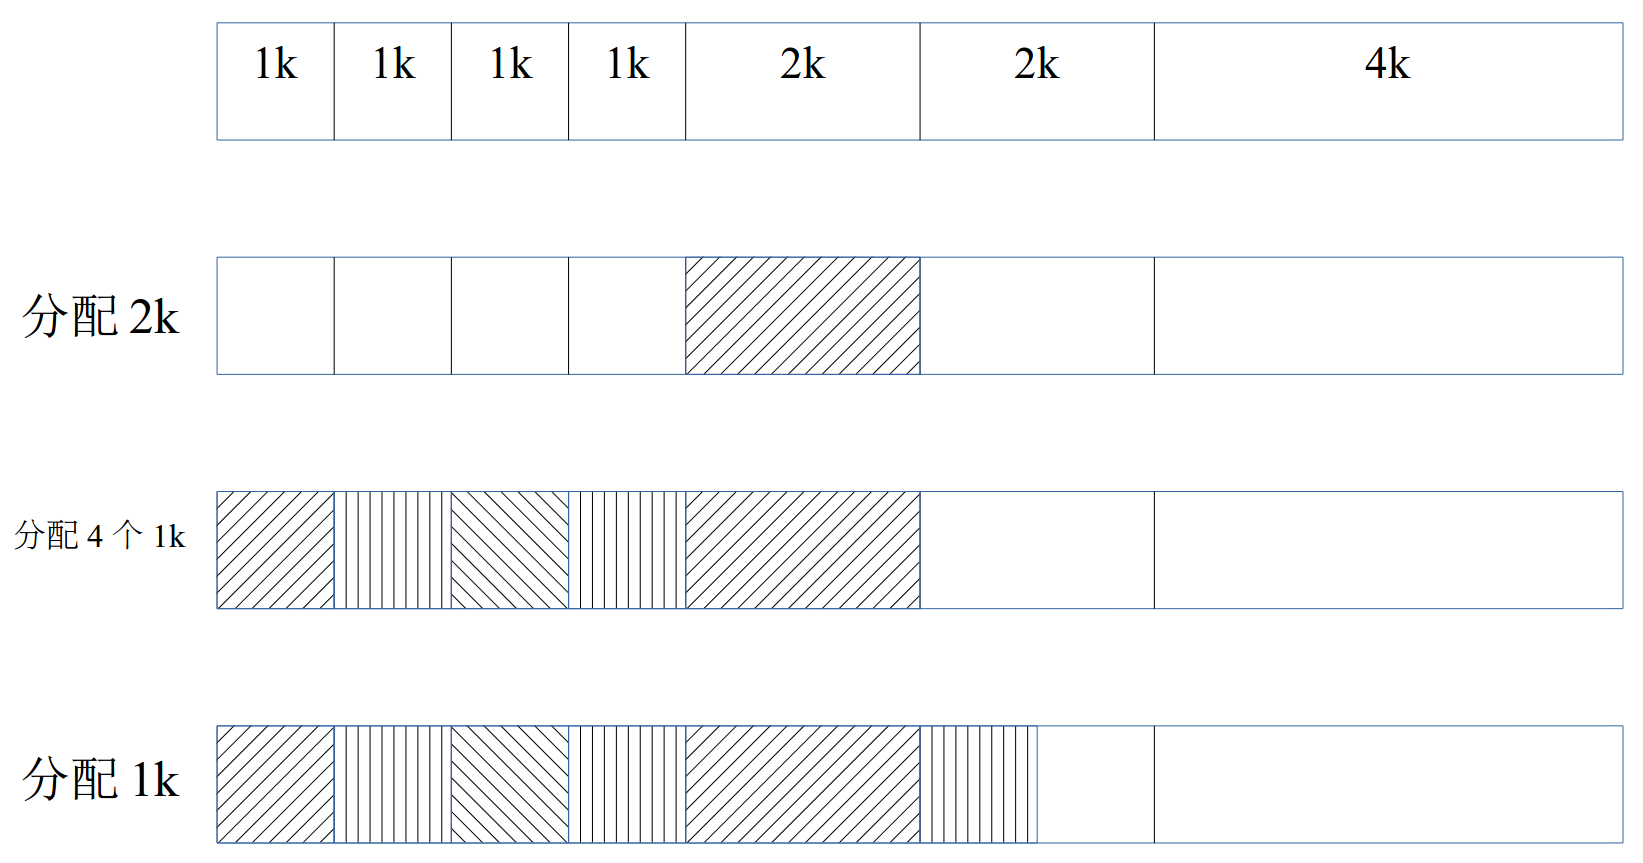
\includegraphics[width = 0.8\textwidth]{memalloc}
		\caption{内存池内存分配实例}
		\label{Figure:Software:memalloc}
	\end{figure}

\subsubsection{内存池的优缺点}
	内存池允许在程序执行时以常数时间分配内存块,并且不会产生内存碎片。一次释放内存中大量空闲内存只需要一个操作,无需像malloc那样依次个别释放。
内存池不必将每次分配的内存的详细信息记录下来(例如内存大小,因为内存池本身就包含了大小的信息)。内存池在使用时也必须按照程序需求来做调整才能保证
时间与空间的效率,这也是内存池的显著缺点。

\subsubsection{内存池在本文中的应用}
	本文所涉及到的算法及所需要的内存大小如表\ref{Tab:Software:Tab1}所示。分析得出内存池需要最多1个32~Bytes,2个128Bytes,6个2048~Bytes和1个8192~Bytes的内存空间。
进一步分析,快速相关以及解调解扩相互间都是独立的,即前一算法执行完毕后一算法才会执行。因此,2048~Bytes的空间只需要2个。为给其他局部变量预留空间,最终的内存池分布为:
16~Bytes$\times$8、32~Bytes$\times$4、128~Bytes$\times$2、256~Bytes$\times$1、2048~Bytes$\times$2、4096~Bytes$\times$1、8192~Bytes$\times$1。

	\begin{table}[htbp]
		\centering 
		\caption{算法内存需求}
		\label{Tab:Software:Tab1}
		\begin{tabular*}{\textwidth}{c|c|c|c}
			\specialrule{1.5pt}{0pt}{0pt}
			% after \\: \hline or \cline{col1-col2} \cline{col3-col4} ...
			算法 & 		数据量 & 数据类型 & 占用空间(Byte) \\
			\hline
			快速相关& 	1024 $\times$ 2 & int16 & 2048 $\times$ 2 \\
			\hline
			\multirow{2}*{解调} & 2048$\times$2 & float32 & 8192$\times$2 \\
							& 512$\times$2  & float32 & 2048 $\times$2\\
			\hline
			\multirow{3}*{解扩与解二阶差分} & 512 $\times$2 & float32 & 2048 $\times$ 2\\
							& 32 $\times$ 2 & float32 & 128 $\times$2 \\
							& 32 $\times$ 1 & int8 & 32 $\times$1 \\
			\specialrule{1.5pt}{0pt}{0pt}
		\end{tabular*}
	\end{table}
	
	
	
	
	